\documentclass{standalone}
\usepackage{tikz}
\begin{document}
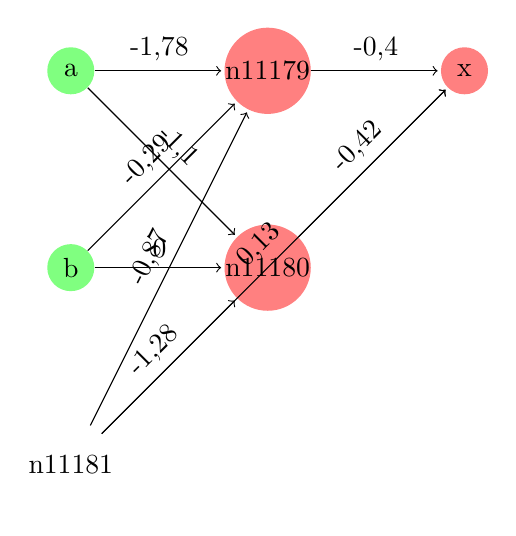
\begin{tikzpicture}[shorten >=1pt,->,draw=black!,node distance=2.5cm]
\tikzstyle{neuron}=[circle,fill=black!25,minimum size=17pt,inner sep=0pt]
\tikzstyle{constant}=[neuron, fill=white!50];
\tikzstyle{sigmoid}=[neuron, fill=red!50];
\tikzstyle{identity}=[neuron, fill=green!50];
\node [identity] (a) {a};
\node [identity,below of=a] (b) {b};
\node [constant,below of=b] (n11181) {n11181};
\node [sigmoid,right of=a] (n11179) {n11179};
\node [sigmoid,below of=n11179] (n11180) {n11180};
\node [sigmoid,right of=n11179] (x) {x};
\path[every node/.style={sloped,anchor=south,auto=false}]
(n11181) edge node {0,13} (x)
(n11181) edge node {-1,28} (n11180)
(n11181) edge node {-0,87} (n11179)
(n11179) edge node {-0,4} (x)
(n11180) edge node {-0,42} (x)
(a) edge node {-1,1} (n11180)
(a) edge node {-1,78} (n11179)
(b) edge node {0} (n11180)
(b) edge node {-0,29} (n11179)
;\end{tikzpicture}
\end{document}